\documentclass[../main.tex]{subfiles}
\begin{document}
\chapter{Soluzione proposta}

In questo capitolo viene presentato il programma di conversione. La prima parte descrive le scelte effettuate per convertire i campi nell'altro formato e come automatizzare la procedura. La seconda parte introduce il concetto di programmazione parallela e le possibili soluzioni per rendere efficiente la conversione.


\section{Conversione}
Per convertire i file di nProbe nel formato utilizzato da Argus si è fatto per prima cosa uno studio sui campi degli header per individuarne le differenze. Alcuni campi sono presenti in entrambi i formati seppure con nome diverso, altri sono stati ottenuti come combinazione, mentre quelli che nProbe utilizza in più rispetto ad Argus sono stati scartati. 

La tabella ~\ref{table:tabellaConversione} mostra sulla colonna di sinistra i campi dell'header di Argus, mentre sulla destra la scelta dei campi di nProbe per rappresentare i dati nello stesso formato scelto da Argus.

\begin{table}[H]
				\centering
				\begin{tabular}{|l|l|}
								\hline
								binetflow												 & flow																								 \\ \hline
								start time											 & first switched																			 \\ \hline
								duration												 & last switched - first switched											 \\ \hline
								protocol												 & protocol																						 \\ \hline
								source address                   & ipv4 source address                                 \\ \hline
								source port                      & source port                                         \\ \hline
								direction                        & biflow direction                                    \\ \hline
								destination address              & ipv4 destination address                            \\ \hline
								destination port                 & destination port                                    \\ \hline
								state                            & -                                                   \\ \hline
								source tos                       & source tos                                          \\ \hline
								destination tos                  & -                                                   \\ \hline
								tot packets                      & input packets + output packets                      \\ \hline
								tot bytes                        & input bytes + output bytes                          \\ \hline
								source bytes                     & input bytes                                         \\ \hline
								source data											 & -																									 \\ \hline
								destination data								 & -																									 \\ \hline
								label														 & -																									 \\ \hline

				\end{tabular}
				\caption{Tabella di conversione}
								\label{table:tabellaConversione}
\end{table}

nProbe e Argus, oltre le differenze degli header presentano anche differenze nel formato con cui sono scritti i file.



\section{Automatizzazione conversione}
La conversione è stata automatizzata con la scrittura di uno script in Python. Si è scelto di scrivere un programma usando questo linguaggio per la facilità di utilizzo nel lavorare con i file e per le performance.

Il problema richiede lo sviluppo di un programma che converte file in modalità batch.
I file hanno una struttura gerarchica per data organizzata per sottocartelle, si esegue quindi un ciclo \textit{for} che prende tutti i file in modo ricorsivo.
Dopodichè si apre il file in lettura leggendo una riga per volta, si converte il contenuto e lo si salva in una lista. Una volta terminata la lettura del file si scrive la lista contente i dati convertiti su un nuovo file.

Si è scelto di leggere il file una riga alla volta perchè le grandi dimensioni dei file non permettono un approccio diverso. Un approccio più veloce sarebbe stato quello di leggere i file per intero nella memoria principale ma non è un approccio possibile perchè possono presentarsi casi in cui la dimensione della RAM, soprattutto nei computer più datati, è più piccola rispetto a quella dei file.

L'algoritmo ~\ref{alg:singleCore} scritto in pseudocodice descrive una soluzione single core al problema

\begin{algorithm}
\caption{Single core version}
				\label{alg:singleCore}
\begin{algorithmic}[1]
\Procedure{Hydra}{}
\ForAll{\textit{file} in path}
\State read data from \textit{file}
\State convert data into new format
\State append data into new file
\EndFor

\EndProcedure
\end{algorithmic}
\end{algorithm}

\section{Rendere efficiente la conversione}

Nel programma descritto in precendenza viene generato un solo file di output in cui vengono convertiti tutti i file dati in input. Questa soluzione è comoda perchè da migliaia di file si ottiene un solo file con i dati convertiti, ma presenta il problema di creare un file con dimensioni enormi e di difficile gestione (il file può raggiungere dimensioni tali da rendere difficile anche solo aprirlo in lettura).


Il programma è inoltre inefficiente poichè è single core e ha come collo di bottiglia la scrittura su un unico file. 
La soluzione proposta seppure sia teoricamente corretta non può avere un'applicazione nel mondo reale. Bisogna cambiare quindi strategia per rendere la conversione più veloce sfruttando le macchine multi core e per avere in output file di dimensioni accettabili.

\subsection{Possibili soluzioni}
Si possono pensare diverse soluzioni che migliorerebbero in modo significativo il programma visto in precedenza:

\begin{itemize}
				\item Lavorare su chunk di file
				\item Meccanismi di lock
				\item Scrittura su file 1:1
\end{itemize}

\begin{verse}
\textbf{Lavorare su chunk di file}
Per velocizzare il programma e sfruttare i processori disponibili si potrebbe assegnare ad ogni processore un file da leggere e convertire. Quando il processore termina la conversione dei dati scrive sul file in output. In questo modo si dividrebbe il tempo di esecuzione sul numero di processori disponibili. 
Questa soluzione rende il più veloce possibile la conversione dei file ma i processori finiscono per scrivere sullo stesso file senza avere nessuna regola di precedenza, questo crea problemi perchè le scritture in output non sono ordinate e non è possibile creare modelli comportamentali affidabili. Le scritture su file devono essere ordinate e sequenziali, inoltre questa soluzione ha il problema di scrivere sempre su unico file e come detto in precedenza questo tipo di soluzione non è possibile.
\end{verse}

\begin{verse}
\textbf{Meccanismi di lock}
Un modo per risolvere i problemi precedenti è quello di utilizzare il concetto di semaforo. 
In informatica un semaforo è un tipo di dato astratto gestito da un sistema operativo multitasking per sincronizzare l'accesso a risorse condivise tra processi. È composto da una variabile intera e da una coda di processi. Quando un processo apre il file per scriverci viene impostato un semaforo che segnala che la risorsa è occupata, se un altro processore prova ad aprire lo stesso file per scriverci gli sarà negato l'accesso dal semaforo fino a quando l'altro processo non rilascerà la risorsa.
In questo modo si risolve il problema delle scritture ordinate, ma c'è da tener conto che i semafori riducono la velocità di esecuzione dell'algoritmo poichè mentre un processore occupa la risorsa tutti gli altri processori devono mettersi in coda per aspettarne il rilascio. Nonostante questa soluzione rallenti l'esecuzione del programma rispetto alla soluzione precedente è comunque molto più veloce della versione single core perchè, sebbene la scrittura su file sia rallentata dai semafori, si guadagna molto tempo nella lettura e conversione dei dati dove non ne è necessario l'utilizzo, e che quindi viene effettuata alla massima velocità possibile. Questa soluzione risolve anche il problema dell'ordinamento delle scritture.
Rimane il problema della scrittura su un unico file che però può essere risolto facilmente decidendo di scrivere su un nuovo file quando raggiunge una dimensione specificata.
Se si implementa la divisione del file di output questa soluzione può considerarsi efficiente anche se rimane il collo di bottiglia introdotto dai semafori che costringe i processi ad aspettare in coda quando una risorsa è impegnata.
\end{verse}

\begin{verse}
\textbf{Scrittura su file 1:1}
In questa soluzione ogni processore apre un file, lo legge, lo converte e scrive su un proprio file.
Questa soluzione è decisamente la più semplice tra quelle proposte ed è anche la più efficiente poichè i processori non entrano mai in conflitto tra di loro cosicchè da effettuare letture, conversioni e scritture alla massima velocità possibile dalla macchina.
Un problema che può creare questa soluzione è la produzione di una grande quantità di file in output. Si pensi che una sola settimana di traffico di rete, sono circa 10 mila file.
\end{verse}

\subsection{Scelta effettuata}

Si è scelto di procedere con l'ultima soluzione presentata perchè data la grande quantità di informazioni da convertire si preferisce l'approccio più veloce a discapito dell'ordinamento finale.

Il programma, dato in input la root directory dei file, cerca ricorsivamente tutti i file e li inserisce in una coda, chiama poi una funzione a cui assegna 4 processori. La funzione ha un ciclo while che si ripete fino a quando la coda popolata da tutti i file non è vuota. Ogni processore che entra in questa funzione toglie un file dalla coda e lo elabora.

Il programma ~\ref{alg:multiCore} descrive una soluzione multi core
\begin{algorithm}
\caption{Multi core version}
				\label{alg:multiCore}
\begin{algorithmic}[1]
\Procedure{Hydra}{}
\ForAll{\textit{file} in path}
\State $\textit{Queue[]} \gets \textit{file}$
\State read data from $\textit{file}$
\State spawn 4 process
\While{\textit{Queue[]} $\textbf{not empty}$}
\State $\textit{filename} \gets $\textit{Queue.get()}
\State convert data into new format
\State append data into new file
\EndWhile
\EndFor
\EndProcedure
\end{algorithmic}
\end{algorithm}
\end{document}

La figura ~\ref{fig:multiCore} descrive lo pseudocodice del programma parallelo. Ogni file da convertire è inserito in una coda a cui accedono i processori, ogni processore lavora individualmente sul proprio file da cui legge e converte i dati. La scrittura su file rimane indipendente perchè ogni processore lavora sul proprio file.

\begin{figure}[H]
				\centering
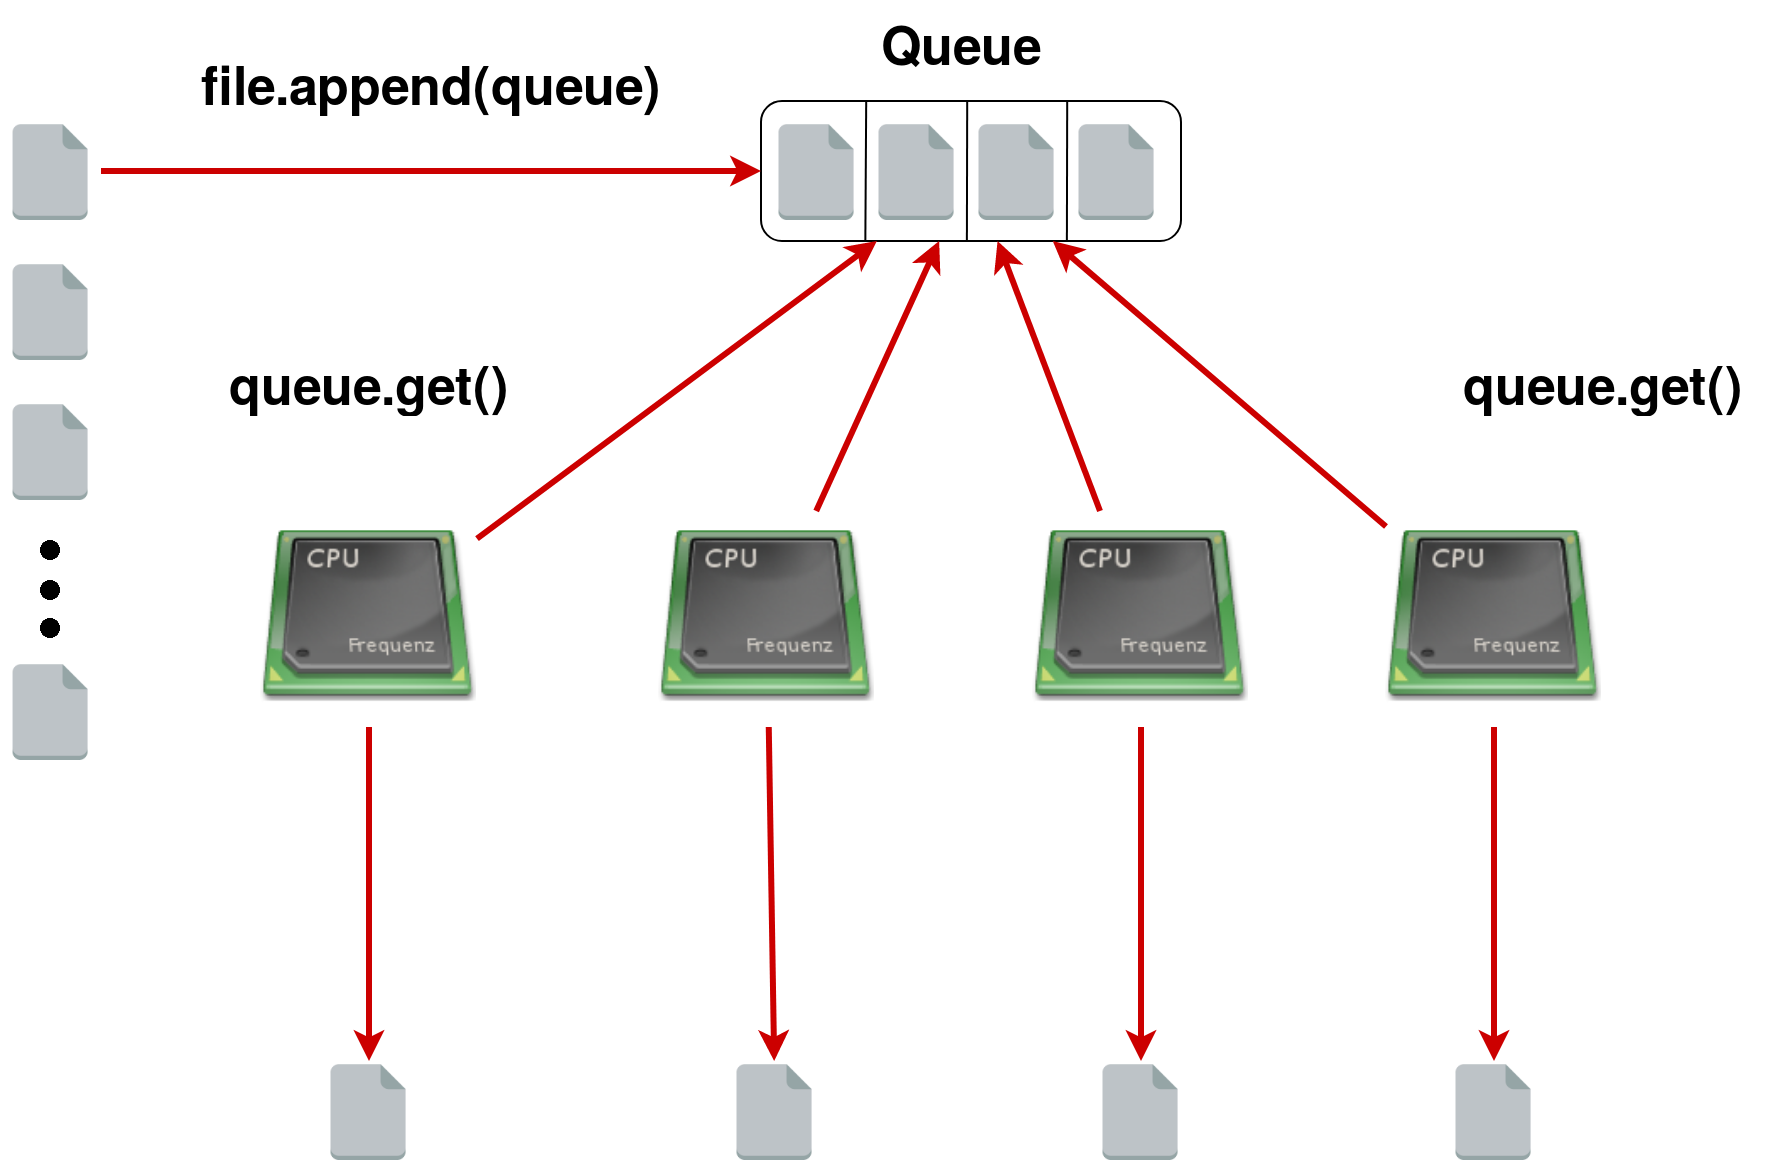
\includegraphics[scale=0.22]{hydra.png}
				\caption{Multi core version}
				\label{fig:multiCore}
\end{figure}


